\section{Simple Algorithm with controlled Memory Layout and Skew}
\label{sec:memorylayout}
In this section, we describe our attempt to improve the query times for the wavelet tree by controlling the memory layout and skewing the tree.
Brodal et al.~\cite{gerthSkewedBinarySearchTrees} showed that skewing a binary search tree could reduce the amount of cache misses and branch mispredictions considerately. Enough, in fact, to increase the speed of searching the tree manyfold, even though the skewing increased the depth of the tree structure.

We want to reduce the number of cache misses in our rank and select queries.
To do this we try and make it so that the next piece of memory the algorithm accesses is already loaded into a cacheline.
One way of doing this is to have the data ordered in memory such that the queries will access them consecutively in memory, as this will mean full utilization of each cacheline as well as enabling prefetching of the next piece of memory to be effective.

We will do this by placing nodes consecutively in memory that are consecutively accessed in a Depth First Search that traverses the right subnode first.

The algorithms remain mostly the same algorithm as the Simple, Naïve approach, but with modifications to handle a controlled memory layout and a skew of the tree.
We have also altered the Naïve approach to support skewing, so we can compare whether the controlled memory layout has the desired effect.

\subsection{Prefetching}
Prefetching is a feature of the CPU whereby it can fetch other parts of the memory into cachelines even though it was not requested yet, if it believes it will be requested soon, to avoid having the program waiting for this fetching.
In more advanced versions, it can even look at the access into memory of the running program and try to determine a pattern and prefetch memory according to this pattern.
Looking at the Intel Optimization Manual~\cite{intel-optimization-manual} for our architecture~\footnote{Our architecture is Ivy Bridge, but the optimization manual sections for Sandy Bridge holds true for Ivy Bridge as well, as stated in section 2.2.7 in \cite{intel-optimization-manual}.} we find that it has a streaming prefetchers loading into L1, L2, and last level cache. The streaming prefetchers detect accesses to ascending or descending addresses and can prefetch up to 20 lines ahead or behind. It also has a prefetcher that can detect strides in memory access, as well as a "Next Page Prefetcher" when detecting memory accesses near the page boundary~\footnote{See section 2.2.7 of ~\cite{intel-optimization-manual}}.


\subsection{Skewing The Tree}
\label{sec:SkewingTheTree}
A way of achieving the sequential memory access in our case would be to skew the entire tree to one side, so that it is most likely that the queries will go to one side for most of the traversal and then control the memory layout so we can put that side of the tree next in memory.
Skewing the tree is done by changing the way we find which character in the alphabet to split on in each node's construction.
The split character is the last character in the alphabet of the left child node and to be able to skew the calculation we calculate it as
\[ \frac{alphabetSize-1}{skew} + alphabetMin \]
where $alphabetSize$ is the size of the alphabet at this node, $alphabetMin$ is the first character in the alphabet at this node, and $skew$ is the skew parameter which is 2 for a balanced tree and higher for skewed trees. E.g. a $skew$ value of 4 will mean we skew the tree by, in each node, putting 25\% of the alphabet into the left child node and 75\% into the right.
Notice also that the division is integer division, meaning anything past the decimal point is thrown away, or in other words, like calling a \texttt{floor()} function on the result of the division.

\subsection{Controlled Memory Layout}
We still want to support dynamic input and alphabet sizes without recompilation, so the nodes must be dynamically allocated on the heap.
It is impossible to know the size of the bitmap of each node before its input string is found by its parent, because the bitmap length in each node is the size of its input string.
Because of this, we cannot store the bitmaps as part of the nodes and neither can we simply use an array of bitmaps to ensure they are in consecutive order in memory.

The size of a node (not including its bitmap) is known at compile time as it contains simply pointers to parent node and left and right child nodes, as well as a boolean to flag it as a leaf node.
As such, we can and do allocate the memory for the nodes by allocating an array, then instantiating nodes into that array.
We pass a reference to a pointer into the array from parent to child nodes during construction, so they know where to allocate their child nodes.
The pointer points to the position of the last node in the array, and so before each instantiation of a new node, we increment the pointer so it points to free space, then place the new node there.

\subsection{Preallocating the Bitmaps}
Because the size of each bitmap is unknown at compile time, we cannot use an array, and so we must do it in another way. We still want the bitmaps stored consecutively in memory and because the bitmaps take up the most space, we would like to ensure that the bits are tightly packed.

We allocate the bitmaps as one giant bitmap the size of the maximum possible size required to store all the bitmaps for all the nodes. The sum of the size of all bitmaps on one layer of the tree can at most be $n$ and we can at most have $h$ layers, so the maximum size becomes
\[n \cdot h\]
where $n$ is the number of characters in the string and $h$ is the max height of a skewed binary tree and is defined in~\cite{Nievergelt:1972:BST:800152.804906} to be:
\[ h = \frac{log(2\sigma+1)}{ log(\frac{1}{1-\frac{1}{skew}})}\]
where $skew$ is the number we divide by to skew our tree.  We then store an offset and a size for the bitmap in each node, so we can index into the giant bitmap and access the bits corresponding to the node.
After having constructed the entire tree, we then shrink the giant bitmap to fit its actual size, to not waste the memory when the tree is in use for querying. Shrinking the bitmap takes less than a microsecond so it does not impact the construction time in any significant way. We use the \texttt{resize()} method to shrink the bitmap to the size of \texttt{bitmapOffset}, the counter that has been incremented to always point at the next free space in the bitmap during the construction and so is also the actual filled size of the bitmap.
If we had allocated a bitmap for each node individually, they would have been word-aligned, and the bits between the end of one bitmap and the start of another would have gone unused and so, wasted.

The nodes now contain, in addition to the previously mentioned pointers, a pointer to the large bitmap, an offset and a size.



\subsection{Experiments}

\subsubsection{Query time when skewing the Wavelet Tree using uncontrolled and controlled memory-layout}

\begin{figure}
\caption{Rank and Select Running times on Wavelet Tree with increasing skew for naive construction and preallocated construction}
\label{fig:NaiveRankSelectSkewRunningTime}
% GNUPLOT: LaTeX picture with Postscript
\begingroup
  \makeatletter
  \providecommand\color[2][]{%
    \GenericError{(gnuplot) \space\space\space\@spaces}{%
      Package color not loaded in conjunction with
      terminal option `colourtext'%
    }{See the gnuplot documentation for explanation.%
    }{Either use 'blacktext' in gnuplot or load the package
      color.sty in LaTeX.}%
    \renewcommand\color[2][]{}%
  }%
  \providecommand\includegraphics[2][]{%
    \GenericError{(gnuplot) \space\space\space\@spaces}{%
      Package graphicx or graphics not loaded%
    }{See the gnuplot documentation for explanation.%
    }{The gnuplot epslatex terminal needs graphicx.sty or graphics.sty.}%
    \renewcommand\includegraphics[2][]{}%
  }%
  \providecommand\rotatebox[2]{#2}%
  \@ifundefined{ifGPcolor}{%
    \newif\ifGPcolor
    \GPcolortrue
  }{}%
  \@ifundefined{ifGPblacktext}{%
    \newif\ifGPblacktext
    \GPblacktexttrue
  }{}%
  % define a \g@addto@macro without @ in the name:
  \let\gplgaddtomacro\g@addto@macro
  % define empty templates for all commands taking text:
  \gdef\gplbacktext{}%
  \gdef\gplfronttext{}%
  \makeatother
  \ifGPblacktext
    % no textcolor at all
    \def\colorrgb#1{}%
    \def\colorgray#1{}%
  \else
    % gray or color?
    \ifGPcolor
      \def\colorrgb#1{\color[rgb]{#1}}%
      \def\colorgray#1{\color[gray]{#1}}%
      \expandafter\def\csname LTw\endcsname{\color{white}}%
      \expandafter\def\csname LTb\endcsname{\color{black}}%
      \expandafter\def\csname LTa\endcsname{\color{black}}%
      \expandafter\def\csname LT0\endcsname{\color[rgb]{1,0,0}}%
      \expandafter\def\csname LT1\endcsname{\color[rgb]{0,1,0}}%
      \expandafter\def\csname LT2\endcsname{\color[rgb]{0,0,1}}%
      \expandafter\def\csname LT3\endcsname{\color[rgb]{1,0,1}}%
      \expandafter\def\csname LT4\endcsname{\color[rgb]{0,1,1}}%
      \expandafter\def\csname LT5\endcsname{\color[rgb]{1,1,0}}%
      \expandafter\def\csname LT6\endcsname{\color[rgb]{0,0,0}}%
      \expandafter\def\csname LT7\endcsname{\color[rgb]{1,0.3,0}}%
      \expandafter\def\csname LT8\endcsname{\color[rgb]{0.5,0.5,0.5}}%
    \else
      % gray
      \def\colorrgb#1{\color{black}}%
      \def\colorgray#1{\color[gray]{#1}}%
      \expandafter\def\csname LTw\endcsname{\color{white}}%
      \expandafter\def\csname LTb\endcsname{\color{black}}%
      \expandafter\def\csname LTa\endcsname{\color{black}}%
      \expandafter\def\csname LT0\endcsname{\color{black}}%
      \expandafter\def\csname LT1\endcsname{\color{black}}%
      \expandafter\def\csname LT2\endcsname{\color{black}}%
      \expandafter\def\csname LT3\endcsname{\color{black}}%
      \expandafter\def\csname LT4\endcsname{\color{black}}%
      \expandafter\def\csname LT5\endcsname{\color{black}}%
      \expandafter\def\csname LT6\endcsname{\color{black}}%
      \expandafter\def\csname LT7\endcsname{\color{black}}%
      \expandafter\def\csname LT8\endcsname{\color{black}}%
    \fi
  \fi
  \setlength{\unitlength}{0.0500bp}%
  \begin{picture}(7200.00,5040.00)%
    \gplgaddtomacro\gplbacktext{%
      \csname LTb\endcsname%
      \put(1342,704){\makebox(0,0)[r]{\strut{} 30000}}%
      \put(1342,1286){\makebox(0,0)[r]{\strut{} 40000}}%
      \put(1342,1867){\makebox(0,0)[r]{\strut{} 50000}}%
      \put(1342,2449){\makebox(0,0)[r]{\strut{} 60000}}%
      \put(1342,3030){\makebox(0,0)[r]{\strut{} 70000}}%
      \put(1342,3612){\makebox(0,0)[r]{\strut{} 80000}}%
      \put(1342,4193){\makebox(0,0)[r]{\strut{} 90000}}%
      \put(1342,4775){\makebox(0,0)[r]{\strut{} 100000}}%
      \put(1474,484){\makebox(0,0){\strut{} 2}}%
      \put(2140,484){\makebox(0,0){\strut{} 3}}%
      \put(2806,484){\makebox(0,0){\strut{} 4}}%
      \put(3472,484){\makebox(0,0){\strut{} 5}}%
      \put(4139,484){\makebox(0,0){\strut{} 6}}%
      \put(4805,484){\makebox(0,0){\strut{} 7}}%
      \put(5471,484){\makebox(0,0){\strut{} 8}}%
      \put(6137,484){\makebox(0,0){\strut{} 9}}%
      \put(6803,484){\makebox(0,0){\strut{} 10}}%
      \put(176,2739){\rotatebox{-270}{\makebox(0,0){\strut{}Wall Time (microsec)}}}%
      \put(4138,154){\makebox(0,0){\strut{}Skew}}%
    }%
    \gplgaddtomacro\gplfronttext{%
      \csname LTb\endcsname%
      \put(3982,4602){\makebox(0,0)[r]{\strut{}NaiveRank}}%
      \csname LTb\endcsname%
      \put(3982,4382){\makebox(0,0)[r]{\strut{}NaiveSelect}}%
      \csname LTb\endcsname%
      \put(3982,4162){\makebox(0,0)[r]{\strut{}PreallocatedRank}}%
      \csname LTb\endcsname%
      \put(3982,3942){\makebox(0,0)[r]{\strut{}PreallocatedSelect}}%
    }%
    \gplbacktext
    \put(0,0){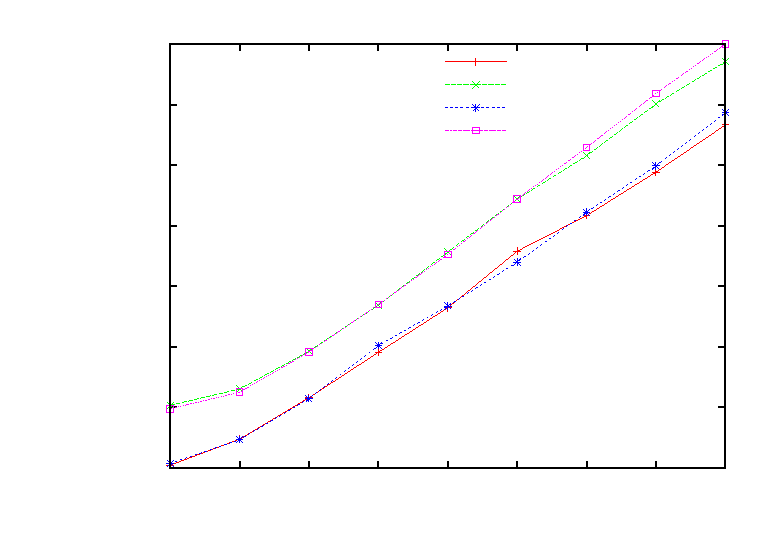
\includegraphics{naiveRankSelectSkewRunningTime}}%
    \gplfronttext
  \end{picture}%
\endgroup

\end{figure}


In this experiment we want to test whether querying our controlled memory version of the Wavelet Tree is faster than querying the uncontrolled memory version for increasingly skewed trees. 

We have run 1000 \texttt{rank} queries and 1000 \texttt{select} queries for each skew and registered the total running time for those 100 queries. 
We did 5 sample runs for each skew and then used the median running time of these. 
This was done to minimize the effect of outliers in the test. The 100 runs was simply done to increase the general size of the running time to better see the differences. The results can be seen in Figure ~\ref{fig:NaiveRankSelectSkewRunningTime}.

We skew the Wavelet Tree (see section~\ref{sec:SkewingTheTree}) because we believe it has better performance than not skewing it since data can then be stored sequentially in memory and reduce cache-misses because of prefetching and should then be faster to access when querying. 
Skewing should also reduce branch mis-predictions since branched to the right become more probable than branching to the left. 


If we look at figure ~\ref{fig:NaiveRankSelectSkewRunningTime} we can see that the query time increases linearly with increasing skew for both controlled and uncontrolled memory layout. We also observe that the two memory layout approaches are almost equal for both rank and select queries in terms of running time.

This means we can conclude that skewing the tree is not an improvement on performance. It is also not an improvement to control the memory our selves.

\subsubsection{Why skewing is not an improvement}
\paragraph{Branch Mis-predictions}
To understand why skewing the tree is no improvement we need to figure out what causes the increase in query time. 
First we look at branch mis-predictions to see if they actually decrease when we increase the skew factor. 
\begin{figure}
\caption{Rank Branch Mis-predictions rate}
\label{fig:NaiveVsPreallocatedSkewRankQueryBMrate}
% GNUPLOT: LaTeX picture with Postscript
\begingroup
  \makeatletter
  \providecommand\color[2][]{%
    \GenericError{(gnuplot) \space\space\space\@spaces}{%
      Package color not loaded in conjunction with
      terminal option `colourtext'%
    }{See the gnuplot documentation for explanation.%
    }{Either use 'blacktext' in gnuplot or load the package
      color.sty in LaTeX.}%
    \renewcommand\color[2][]{}%
  }%
  \providecommand\includegraphics[2][]{%
    \GenericError{(gnuplot) \space\space\space\@spaces}{%
      Package graphicx or graphics not loaded%
    }{See the gnuplot documentation for explanation.%
    }{The gnuplot epslatex terminal needs graphicx.sty or graphics.sty.}%
    \renewcommand\includegraphics[2][]{}%
  }%
  \providecommand\rotatebox[2]{#2}%
  \@ifundefined{ifGPcolor}{%
    \newif\ifGPcolor
    \GPcolortrue
  }{}%
  \@ifundefined{ifGPblacktext}{%
    \newif\ifGPblacktext
    \GPblacktexttrue
  }{}%
  % define a \g@addto@macro without @ in the name:
  \let\gplgaddtomacro\g@addto@macro
  % define empty templates for all commands taking text:
  \gdef\gplbacktext{}%
  \gdef\gplfronttext{}%
  \makeatother
  \ifGPblacktext
    % no textcolor at all
    \def\colorrgb#1{}%
    \def\colorgray#1{}%
  \else
    % gray or color?
    \ifGPcolor
      \def\colorrgb#1{\color[rgb]{#1}}%
      \def\colorgray#1{\color[gray]{#1}}%
      \expandafter\def\csname LTw\endcsname{\color{white}}%
      \expandafter\def\csname LTb\endcsname{\color{black}}%
      \expandafter\def\csname LTa\endcsname{\color{black}}%
      \expandafter\def\csname LT0\endcsname{\color[rgb]{1,0,0}}%
      \expandafter\def\csname LT1\endcsname{\color[rgb]{0,1,0}}%
      \expandafter\def\csname LT2\endcsname{\color[rgb]{0,0,1}}%
      \expandafter\def\csname LT3\endcsname{\color[rgb]{1,0,1}}%
      \expandafter\def\csname LT4\endcsname{\color[rgb]{0,1,1}}%
      \expandafter\def\csname LT5\endcsname{\color[rgb]{1,1,0}}%
      \expandafter\def\csname LT6\endcsname{\color[rgb]{0,0,0}}%
      \expandafter\def\csname LT7\endcsname{\color[rgb]{1,0.3,0}}%
      \expandafter\def\csname LT8\endcsname{\color[rgb]{0.5,0.5,0.5}}%
    \else
      % gray
      \def\colorrgb#1{\color{black}}%
      \def\colorgray#1{\color[gray]{#1}}%
      \expandafter\def\csname LTw\endcsname{\color{white}}%
      \expandafter\def\csname LTb\endcsname{\color{black}}%
      \expandafter\def\csname LTa\endcsname{\color{black}}%
      \expandafter\def\csname LT0\endcsname{\color{black}}%
      \expandafter\def\csname LT1\endcsname{\color{black}}%
      \expandafter\def\csname LT2\endcsname{\color{black}}%
      \expandafter\def\csname LT3\endcsname{\color{black}}%
      \expandafter\def\csname LT4\endcsname{\color{black}}%
      \expandafter\def\csname LT5\endcsname{\color{black}}%
      \expandafter\def\csname LT6\endcsname{\color{black}}%
      \expandafter\def\csname LT7\endcsname{\color{black}}%
      \expandafter\def\csname LT8\endcsname{\color{black}}%
    \fi
  \fi
  \setlength{\unitlength}{0.0500bp}%
  \begin{picture}(7200.00,5040.00)%
    \gplgaddtomacro\gplbacktext{%
      \csname LTb\endcsname%
      \put(1342,704){\makebox(0,0)[r]{\strut{}0.00005}}%
      \put(1342,1383){\makebox(0,0)[r]{\strut{}0.00006}}%
      \put(1342,2061){\makebox(0,0)[r]{\strut{}0.00007}}%
      \put(1342,2740){\makebox(0,0)[r]{\strut{}0.00008}}%
      \put(1342,3418){\makebox(0,0)[r]{\strut{}0.00009}}%
      \put(1342,4097){\makebox(0,0)[r]{\strut{}0.00010}}%
      \put(1342,4775){\makebox(0,0)[r]{\strut{}0.00011}}%
      \put(1474,484){\makebox(0,0){\strut{} 2}}%
      \put(2235,484){\makebox(0,0){\strut{} 4}}%
      \put(2997,484){\makebox(0,0){\strut{} 6}}%
      \put(3758,484){\makebox(0,0){\strut{} 8}}%
      \put(4519,484){\makebox(0,0){\strut{} 10}}%
      \put(5280,484){\makebox(0,0){\strut{} 12}}%
      \put(6042,484){\makebox(0,0){\strut{} 14}}%
      \put(6803,484){\makebox(0,0){\strut{} 16}}%
      \put(176,2739){\rotatebox{-270}{\makebox(0,0){\strut{}Branch mis-prediction rate}}}%
      \put(4138,154){\makebox(0,0){\strut{}Skew}}%
    }%
    \gplgaddtomacro\gplfronttext{%
      \csname LTb\endcsname%
      \put(3190,4602){\makebox(0,0)[r]{\strut{}Naive}}%
      \csname LTb\endcsname%
      \put(3190,4382){\makebox(0,0)[r]{\strut{}Preallocated}}%
    }%
    \gplbacktext
    \put(0,0){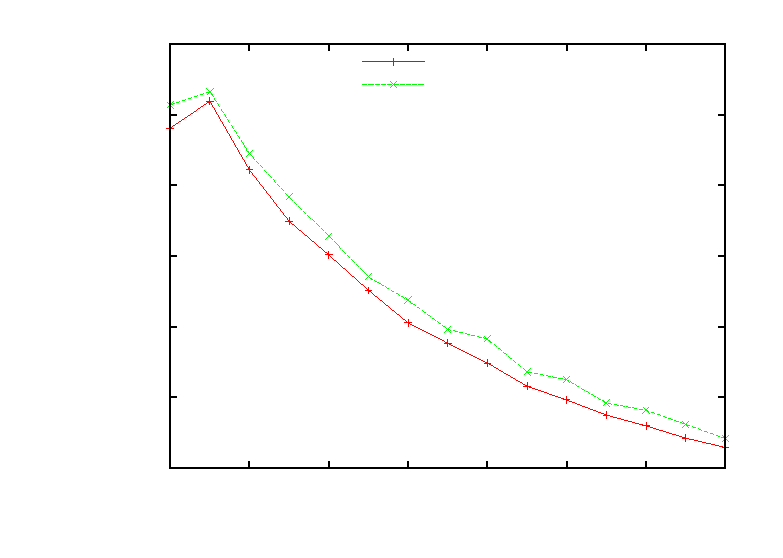
\includegraphics{NaiveVsPreallocatedSkewRankQuery_BR_CN}}%
    \gplfronttext
  \end{picture}%
\endgroup

\end{figure}

\begin{figure}
\caption{Select Branch Mis-predictions rate}
\label{fig:NaiveVsPreallocatedSkewSelectQueryBMrate}
% GNUPLOT: LaTeX picture with Postscript
\begingroup
  \makeatletter
  \providecommand\color[2][]{%
    \GenericError{(gnuplot) \space\space\space\@spaces}{%
      Package color not loaded in conjunction with
      terminal option `colourtext'%
    }{See the gnuplot documentation for explanation.%
    }{Either use 'blacktext' in gnuplot or load the package
      color.sty in LaTeX.}%
    \renewcommand\color[2][]{}%
  }%
  \providecommand\includegraphics[2][]{%
    \GenericError{(gnuplot) \space\space\space\@spaces}{%
      Package graphicx or graphics not loaded%
    }{See the gnuplot documentation for explanation.%
    }{The gnuplot epslatex terminal needs graphicx.sty or graphics.sty.}%
    \renewcommand\includegraphics[2][]{}%
  }%
  \providecommand\rotatebox[2]{#2}%
  \@ifundefined{ifGPcolor}{%
    \newif\ifGPcolor
    \GPcolortrue
  }{}%
  \@ifundefined{ifGPblacktext}{%
    \newif\ifGPblacktext
    \GPblacktexttrue
  }{}%
  % define a \g@addto@macro without @ in the name:
  \let\gplgaddtomacro\g@addto@macro
  % define empty templates for all commands taking text:
  \gdef\gplbacktext{}%
  \gdef\gplfronttext{}%
  \makeatother
  \ifGPblacktext
    % no textcolor at all
    \def\colorrgb#1{}%
    \def\colorgray#1{}%
  \else
    % gray or color?
    \ifGPcolor
      \def\colorrgb#1{\color[rgb]{#1}}%
      \def\colorgray#1{\color[gray]{#1}}%
      \expandafter\def\csname LTw\endcsname{\color{white}}%
      \expandafter\def\csname LTb\endcsname{\color{black}}%
      \expandafter\def\csname LTa\endcsname{\color{black}}%
      \expandafter\def\csname LT0\endcsname{\color[rgb]{1,0,0}}%
      \expandafter\def\csname LT1\endcsname{\color[rgb]{0,1,0}}%
      \expandafter\def\csname LT2\endcsname{\color[rgb]{0,0,1}}%
      \expandafter\def\csname LT3\endcsname{\color[rgb]{1,0,1}}%
      \expandafter\def\csname LT4\endcsname{\color[rgb]{0,1,1}}%
      \expandafter\def\csname LT5\endcsname{\color[rgb]{1,1,0}}%
      \expandafter\def\csname LT6\endcsname{\color[rgb]{0,0,0}}%
      \expandafter\def\csname LT7\endcsname{\color[rgb]{1,0.3,0}}%
      \expandafter\def\csname LT8\endcsname{\color[rgb]{0.5,0.5,0.5}}%
    \else
      % gray
      \def\colorrgb#1{\color{black}}%
      \def\colorgray#1{\color[gray]{#1}}%
      \expandafter\def\csname LTw\endcsname{\color{white}}%
      \expandafter\def\csname LTb\endcsname{\color{black}}%
      \expandafter\def\csname LTa\endcsname{\color{black}}%
      \expandafter\def\csname LT0\endcsname{\color{black}}%
      \expandafter\def\csname LT1\endcsname{\color{black}}%
      \expandafter\def\csname LT2\endcsname{\color{black}}%
      \expandafter\def\csname LT3\endcsname{\color{black}}%
      \expandafter\def\csname LT4\endcsname{\color{black}}%
      \expandafter\def\csname LT5\endcsname{\color{black}}%
      \expandafter\def\csname LT6\endcsname{\color{black}}%
      \expandafter\def\csname LT7\endcsname{\color{black}}%
      \expandafter\def\csname LT8\endcsname{\color{black}}%
    \fi
  \fi
  \setlength{\unitlength}{0.0500bp}%
  \begin{picture}(7200.00,5040.00)%
    \gplgaddtomacro\gplbacktext{%
      \csname LTb\endcsname%
      \put(1474,704){\makebox(0,0)[r]{\strut{} 5e-05}}%
      \put(1474,1156){\makebox(0,0)[r]{\strut{} 0.0001}}%
      \put(1474,1609){\makebox(0,0)[r]{\strut{} 0.00015}}%
      \put(1474,2061){\makebox(0,0)[r]{\strut{} 0.0002}}%
      \put(1474,2513){\makebox(0,0)[r]{\strut{} 0.00025}}%
      \put(1474,2966){\makebox(0,0)[r]{\strut{} 0.0003}}%
      \put(1474,3418){\makebox(0,0)[r]{\strut{} 0.00035}}%
      \put(1474,3870){\makebox(0,0)[r]{\strut{} 0.0004}}%
      \put(1474,4323){\makebox(0,0)[r]{\strut{} 0.00045}}%
      \put(1474,4775){\makebox(0,0)[r]{\strut{} 0.0005}}%
      \put(1606,484){\makebox(0,0){\strut{} 2}}%
      \put(2348,484){\makebox(0,0){\strut{} 4}}%
      \put(3091,484){\makebox(0,0){\strut{} 6}}%
      \put(3833,484){\makebox(0,0){\strut{} 8}}%
      \put(4576,484){\makebox(0,0){\strut{} 10}}%
      \put(5318,484){\makebox(0,0){\strut{} 12}}%
      \put(6061,484){\makebox(0,0){\strut{} 14}}%
      \put(6803,484){\makebox(0,0){\strut{} 16}}%
      \put(176,2739){\rotatebox{-270}{\makebox(0,0){\strut{}Branch mis-prediction rate}}}%
      \put(4204,154){\makebox(0,0){\strut{}Skew}}%
    }%
    \gplgaddtomacro\gplfronttext{%
      \csname LTb\endcsname%
      \put(3322,4602){\makebox(0,0)[r]{\strut{}Naive}}%
      \csname LTb\endcsname%
      \put(3322,4382){\makebox(0,0)[r]{\strut{}Preallocated}}%
    }%
    \gplbacktext
    \put(0,0){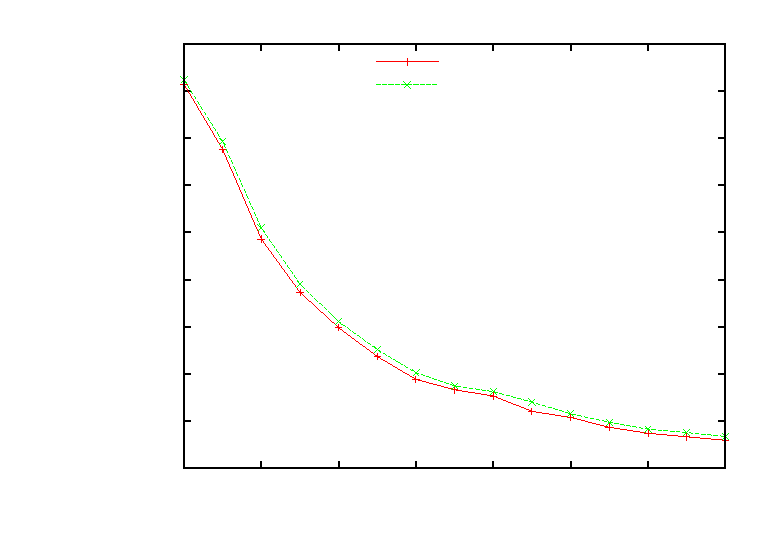
\includegraphics{NaiveVsPreallocatedSkewSelectQuery_BR_CN}}%
    \gplfronttext
  \end{picture}%
\endgroup

\end{figure}
 
Figure ~\ref{fig:NaiveVsPreallocatedSkewRankQueryBMrate} and \ref{fig:NaiveVsPreallocatedSkewSelectQueryBMrate} shows the branch mis-prediction rate for rank and select queries on a wavelet tree with increasing skew factor for both the controlled and uncontrolled memory approach. 
The branch mis-prediction rate is calculated by dividing the number of branch mis-predictions with the total number of conditional branches.

We observe that the branch mis-prediction rate is decreasing as we expected. 
This means that it is not branch mis-predictions that causes the increase in query time. 


\paragraph{Cache misses}
We now look at cache misses to see if they can explain the increase in query time. 
The values are shown in Figure ~\ref{fig:NaivePreallocatedRankSkewCacheMisses} for \texttt{Rank} and in Figure ~\ref{fig:NaivePreallocatedSelectSkewCacheMisses} for \texttt{Select}.
The same tendency as in Figure ~\ref{fig:NaiveRankSelectSkewRunningTime} is observed: 
The cache misses also increases linearly with the skew factor which could explain the linear increase in query time when skewing the tree.

It makes sense that cache misses are increasing because we are accessing a large bitmap in most of the nodes in the tree, that cannot fit in the cache if we are working on large enough data.
Skewing the tree should decrease cache misses because of cache prefetching, but because rank and select stops at some position inside the bitmap and then continues to the next bitmap in the next node it means that they do not gain much advantage from prefetching because the prefetched data in many cases are just the rest of the current bitmap. 
The problem is shown in figure ~\ref{fig:QueryPrefetchFigure}. The bitmap is stored sequentially and the prefetcher prefetches the next cache line which consists of a number of words containing data of the current bitmap.
Rank or select loops through each word in the current cache line and stops somewhere inside a word and continues to the bitmap of the next node and skips the data in the prefetched cache line of the current bitmap.

\begin{figure}
\caption{Why concatenating bitmaps doesn't enable cache prefetching}
\label{fig:QueryPrefetchFigure}
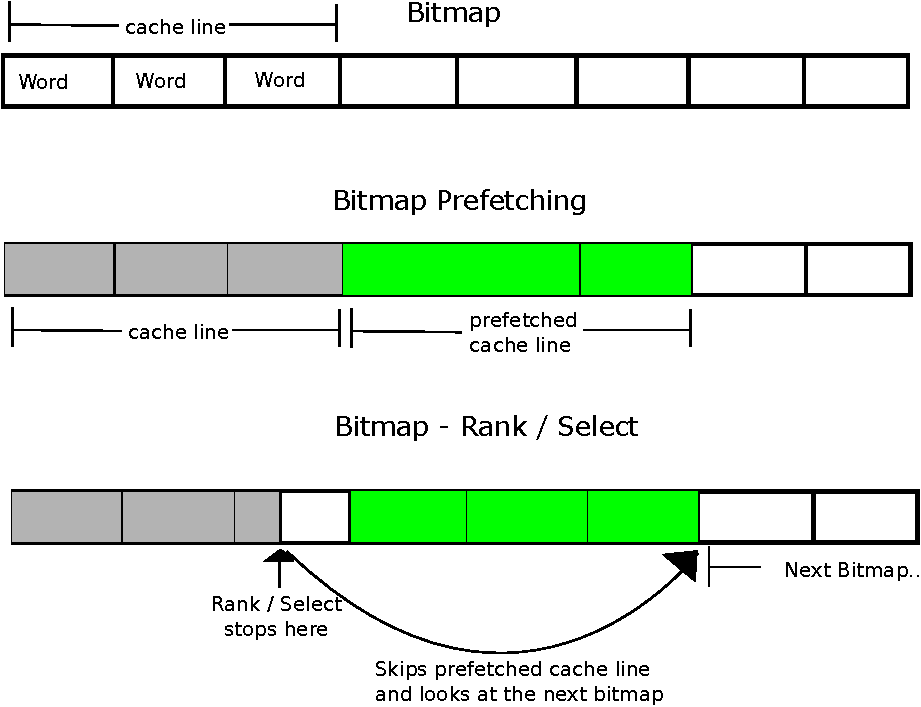
\includegraphics[width=\textwidth]{QueryPrefetchFigure.pdf}
\end{figure}

Prefetching then only helps in the cases where the last entry of the current bitmap is the position where rank or select stops, which does not happen very often.
A cache miss then happens almost every time the select or rank query looks at a new node, until we reach a level of the tree where the bitmap has become small enough to not fill up the cache, which might not happen at all since there can be so many occurrences of even a single character that it allows the bitmap to still be too large to fit in the cache even in the lower levels of the tree.
When we skew the tree we do not split the alphabet into equal sizes anymore and therefore add more data to the right side of the tree than to the left. 
This increases the hight of the tree and we need to look at more nodes to find the result than if the tree was balanced and as a result this we introduce more cache misses because we have to access more bitmaps.
Increasing the height of the tree also generally increases the query time because there are more levels to search through than in a balanced tree.

This is why the query time increases when we skew the tree: we get more cache misses and we have to search through more levels of the tree. 
This suggests that skewing the tree can be an improvement when taking advantage of prefetching is possible and/or when a node only has to access small data that can be kept in cache.

\begin{figure}
\caption{Rank Cache Misses on Wavelet Tree with increasing skew}
\label{fig:NaivePreallocatedRankSkewCacheMisses}
\centering
\begin{subfigure}{\textwidth}
	\caption{Naive L1 vs. Preallocated L1}
	\label{fig:L1NaivePreallocatedRankSkewCacheMisses}
	% GNUPLOT: LaTeX picture with Postscript
\begingroup
  \makeatletter
  \providecommand\color[2][]{%
    \GenericError{(gnuplot) \space\space\space\@spaces}{%
      Package color not loaded in conjunction with
      terminal option `colourtext'%
    }{See the gnuplot documentation for explanation.%
    }{Either use 'blacktext' in gnuplot or load the package
      color.sty in LaTeX.}%
    \renewcommand\color[2][]{}%
  }%
  \providecommand\includegraphics[2][]{%
    \GenericError{(gnuplot) \space\space\space\@spaces}{%
      Package graphicx or graphics not loaded%
    }{See the gnuplot documentation for explanation.%
    }{The gnuplot epslatex terminal needs graphicx.sty or graphics.sty.}%
    \renewcommand\includegraphics[2][]{}%
  }%
  \providecommand\rotatebox[2]{#2}%
  \@ifundefined{ifGPcolor}{%
    \newif\ifGPcolor
    \GPcolortrue
  }{}%
  \@ifundefined{ifGPblacktext}{%
    \newif\ifGPblacktext
    \GPblacktexttrue
  }{}%
  % define a \g@addto@macro without @ in the name:
  \let\gplgaddtomacro\g@addto@macro
  % define empty templates for all commands taking text:
  \gdef\gplbacktext{}%
  \gdef\gplfronttext{}%
  \makeatother
  \ifGPblacktext
    % no textcolor at all
    \def\colorrgb#1{}%
    \def\colorgray#1{}%
  \else
    % gray or color?
    \ifGPcolor
      \def\colorrgb#1{\color[rgb]{#1}}%
      \def\colorgray#1{\color[gray]{#1}}%
      \expandafter\def\csname LTw\endcsname{\color{white}}%
      \expandafter\def\csname LTb\endcsname{\color{black}}%
      \expandafter\def\csname LTa\endcsname{\color{black}}%
      \expandafter\def\csname LT0\endcsname{\color[rgb]{1,0,0}}%
      \expandafter\def\csname LT1\endcsname{\color[rgb]{0,1,0}}%
      \expandafter\def\csname LT2\endcsname{\color[rgb]{0,0,1}}%
      \expandafter\def\csname LT3\endcsname{\color[rgb]{1,0,1}}%
      \expandafter\def\csname LT4\endcsname{\color[rgb]{0,1,1}}%
      \expandafter\def\csname LT5\endcsname{\color[rgb]{1,1,0}}%
      \expandafter\def\csname LT6\endcsname{\color[rgb]{0,0,0}}%
      \expandafter\def\csname LT7\endcsname{\color[rgb]{1,0.3,0}}%
      \expandafter\def\csname LT8\endcsname{\color[rgb]{0.5,0.5,0.5}}%
    \else
      % gray
      \def\colorrgb#1{\color{black}}%
      \def\colorgray#1{\color[gray]{#1}}%
      \expandafter\def\csname LTw\endcsname{\color{white}}%
      \expandafter\def\csname LTb\endcsname{\color{black}}%
      \expandafter\def\csname LTa\endcsname{\color{black}}%
      \expandafter\def\csname LT0\endcsname{\color{black}}%
      \expandafter\def\csname LT1\endcsname{\color{black}}%
      \expandafter\def\csname LT2\endcsname{\color{black}}%
      \expandafter\def\csname LT3\endcsname{\color{black}}%
      \expandafter\def\csname LT4\endcsname{\color{black}}%
      \expandafter\def\csname LT5\endcsname{\color{black}}%
      \expandafter\def\csname LT6\endcsname{\color{black}}%
      \expandafter\def\csname LT7\endcsname{\color{black}}%
      \expandafter\def\csname LT8\endcsname{\color{black}}%
    \fi
  \fi
  \setlength{\unitlength}{0.0500bp}%
  \begin{picture}(7200.00,5040.00)%
    \gplgaddtomacro\gplbacktext{%
      \csname LTb\endcsname%
      \put(1474,704){\makebox(0,0)[r]{\strut{} 3e+06}}%
      \put(1474,1213){\makebox(0,0)[r]{\strut{} 4e+06}}%
      \put(1474,1722){\makebox(0,0)[r]{\strut{} 5e+06}}%
      \put(1474,2231){\makebox(0,0)[r]{\strut{} 6e+06}}%
      \put(1474,2740){\makebox(0,0)[r]{\strut{} 7e+06}}%
      \put(1474,3248){\makebox(0,0)[r]{\strut{} 8e+06}}%
      \put(1474,3757){\makebox(0,0)[r]{\strut{} 9e+06}}%
      \put(1474,4266){\makebox(0,0)[r]{\strut{} 1e+07}}%
      \put(1474,4775){\makebox(0,0)[r]{\strut{} 1.1e+07}}%
      \put(1606,484){\makebox(0,0){\strut{} 2}}%
      \put(2256,484){\makebox(0,0){\strut{} 3}}%
      \put(2905,484){\makebox(0,0){\strut{} 4}}%
      \put(3555,484){\makebox(0,0){\strut{} 5}}%
      \put(4205,484){\makebox(0,0){\strut{} 6}}%
      \put(4854,484){\makebox(0,0){\strut{} 7}}%
      \put(5504,484){\makebox(0,0){\strut{} 8}}%
      \put(6153,484){\makebox(0,0){\strut{} 9}}%
      \put(6803,484){\makebox(0,0){\strut{} 10}}%
      \put(176,2739){\rotatebox{-270}{\makebox(0,0){\strut{}Cache Misses}}}%
      \put(4204,154){\makebox(0,0){\strut{}Skew}}%
    }%
    \gplgaddtomacro\gplfronttext{%
      \csname LTb\endcsname%
      \put(3718,4602){\makebox(0,0)[r]{\strut{}Naive L1}}%
      \csname LTb\endcsname%
      \put(3718,4382){\makebox(0,0)[r]{\strut{}Preallocated L1}}%
    }%
    \gplbacktext
    \put(0,0){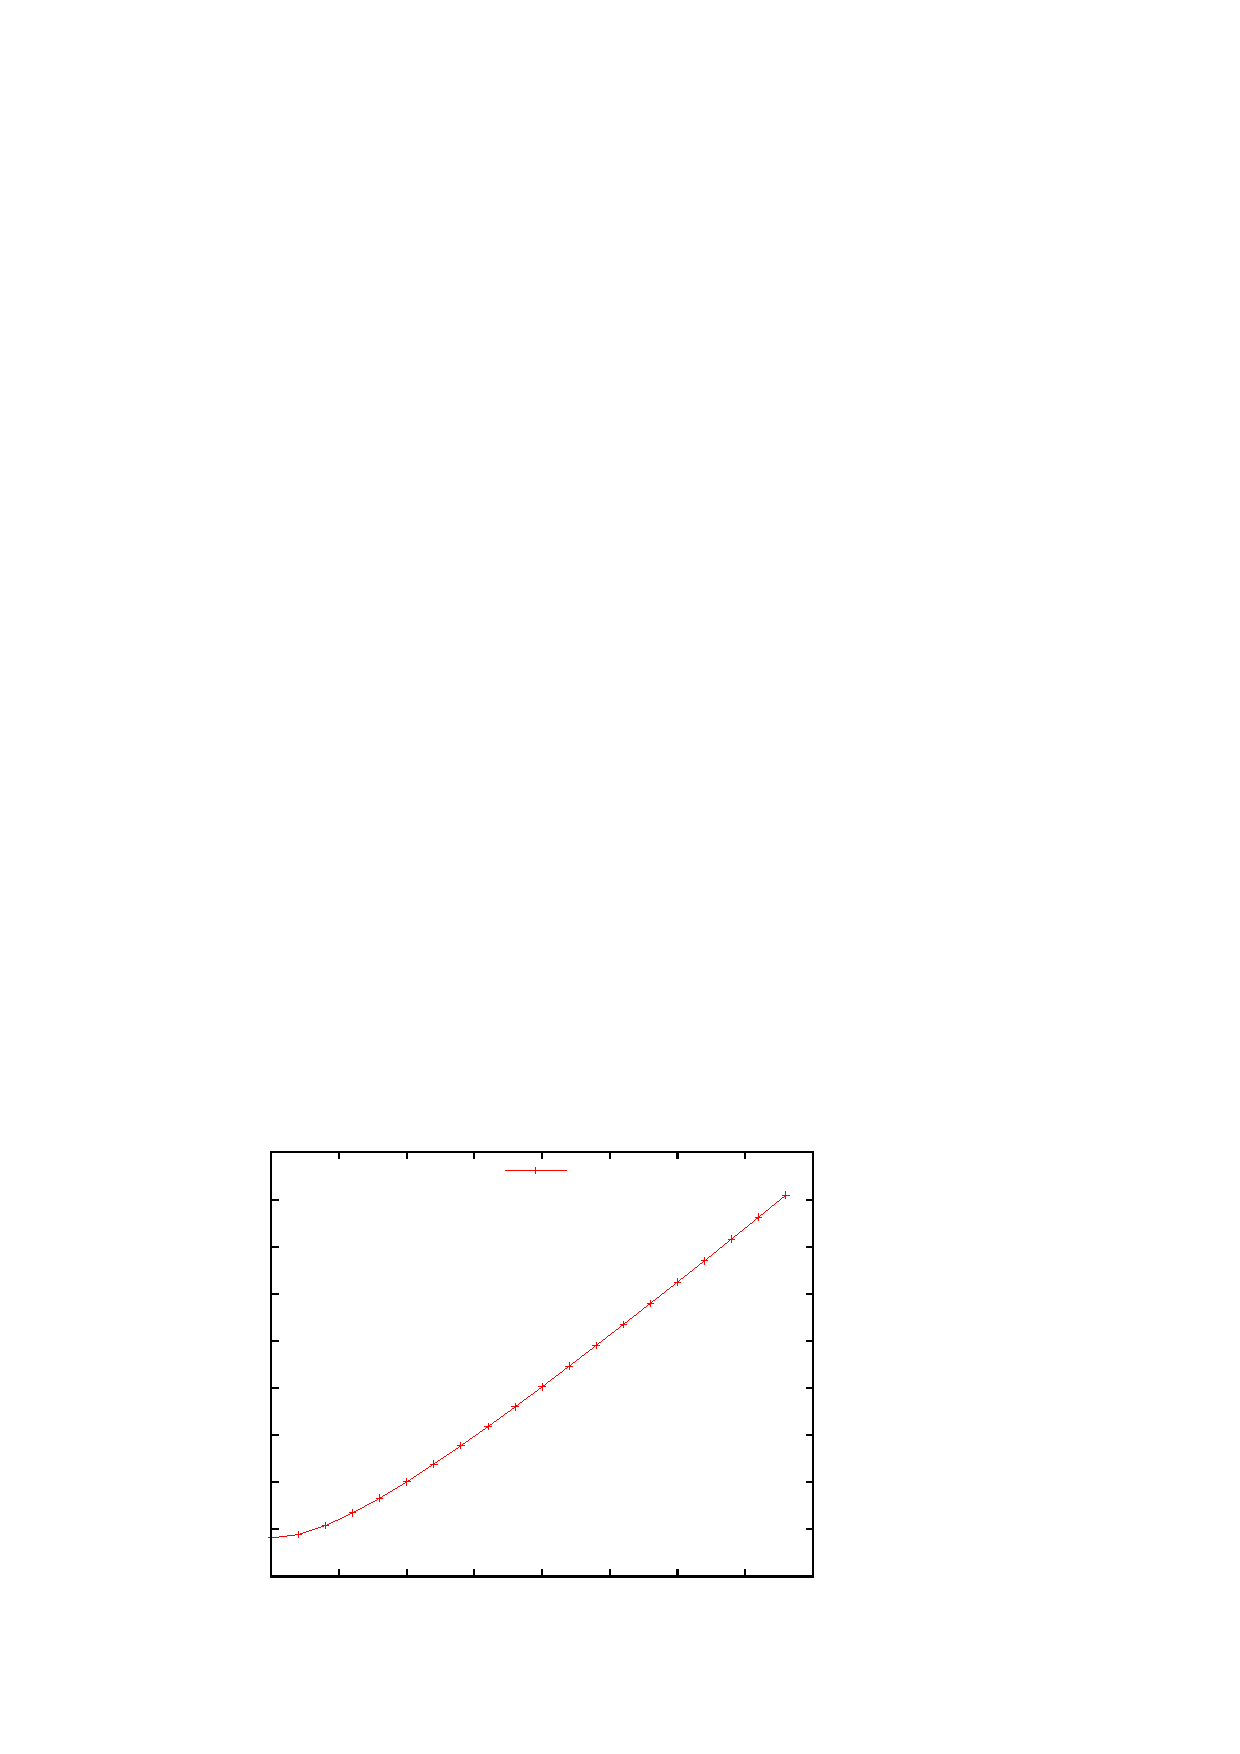
\includegraphics{L1NaiveVsPreallocatedSkewRankQueryCacheMisses}}%
    \gplfronttext
  \end{picture}%
\endgroup

	\vspace*{5 mm}
\end{subfigure}
\begin{subfigure}{\textwidth}
	\caption{Naive L2, L3 vs. Preallocated L2, L3}
	\label{fig:L2L3NaivePreallocatedRankSkewCacheMisses}
 	% GNUPLOT: LaTeX picture with Postscript
\begingroup
  \makeatletter
  \providecommand\color[2][]{%
    \GenericError{(gnuplot) \space\space\space\@spaces}{%
      Package color not loaded in conjunction with
      terminal option `colourtext'%
    }{See the gnuplot documentation for explanation.%
    }{Either use 'blacktext' in gnuplot or load the package
      color.sty in LaTeX.}%
    \renewcommand\color[2][]{}%
  }%
  \providecommand\includegraphics[2][]{%
    \GenericError{(gnuplot) \space\space\space\@spaces}{%
      Package graphicx or graphics not loaded%
    }{See the gnuplot documentation for explanation.%
    }{The gnuplot epslatex terminal needs graphicx.sty or graphics.sty.}%
    \renewcommand\includegraphics[2][]{}%
  }%
  \providecommand\rotatebox[2]{#2}%
  \@ifundefined{ifGPcolor}{%
    \newif\ifGPcolor
    \GPcolortrue
  }{}%
  \@ifundefined{ifGPblacktext}{%
    \newif\ifGPblacktext
    \GPblacktexttrue
  }{}%
  % define a \g@addto@macro without @ in the name:
  \let\gplgaddtomacro\g@addto@macro
  % define empty templates for all commands taking text:
  \gdef\gplbacktext{}%
  \gdef\gplfronttext{}%
  \makeatother
  \ifGPblacktext
    % no textcolor at all
    \def\colorrgb#1{}%
    \def\colorgray#1{}%
  \else
    % gray or color?
    \ifGPcolor
      \def\colorrgb#1{\color[rgb]{#1}}%
      \def\colorgray#1{\color[gray]{#1}}%
      \expandafter\def\csname LTw\endcsname{\color{white}}%
      \expandafter\def\csname LTb\endcsname{\color{black}}%
      \expandafter\def\csname LTa\endcsname{\color{black}}%
      \expandafter\def\csname LT0\endcsname{\color[rgb]{1,0,0}}%
      \expandafter\def\csname LT1\endcsname{\color[rgb]{0,1,0}}%
      \expandafter\def\csname LT2\endcsname{\color[rgb]{0,0,1}}%
      \expandafter\def\csname LT3\endcsname{\color[rgb]{1,0,1}}%
      \expandafter\def\csname LT4\endcsname{\color[rgb]{0,1,1}}%
      \expandafter\def\csname LT5\endcsname{\color[rgb]{1,1,0}}%
      \expandafter\def\csname LT6\endcsname{\color[rgb]{0,0,0}}%
      \expandafter\def\csname LT7\endcsname{\color[rgb]{1,0.3,0}}%
      \expandafter\def\csname LT8\endcsname{\color[rgb]{0.5,0.5,0.5}}%
    \else
      % gray
      \def\colorrgb#1{\color{black}}%
      \def\colorgray#1{\color[gray]{#1}}%
      \expandafter\def\csname LTw\endcsname{\color{white}}%
      \expandafter\def\csname LTb\endcsname{\color{black}}%
      \expandafter\def\csname LTa\endcsname{\color{black}}%
      \expandafter\def\csname LT0\endcsname{\color{black}}%
      \expandafter\def\csname LT1\endcsname{\color{black}}%
      \expandafter\def\csname LT2\endcsname{\color{black}}%
      \expandafter\def\csname LT3\endcsname{\color{black}}%
      \expandafter\def\csname LT4\endcsname{\color{black}}%
      \expandafter\def\csname LT5\endcsname{\color{black}}%
      \expandafter\def\csname LT6\endcsname{\color{black}}%
      \expandafter\def\csname LT7\endcsname{\color{black}}%
      \expandafter\def\csname LT8\endcsname{\color{black}}%
    \fi
  \fi
  \setlength{\unitlength}{0.0500bp}%
  \begin{picture}(7200.00,5040.00)%
    \gplgaddtomacro\gplbacktext{%
      \csname LTb\endcsname%
      \put(1474,704){\makebox(0,0)[r]{\strut{} 0}}%
      \put(1474,1213){\makebox(0,0)[r]{\strut{} 200000}}%
      \put(1474,1722){\makebox(0,0)[r]{\strut{} 400000}}%
      \put(1474,2231){\makebox(0,0)[r]{\strut{} 600000}}%
      \put(1474,2740){\makebox(0,0)[r]{\strut{} 800000}}%
      \put(1474,3248){\makebox(0,0)[r]{\strut{} 1e+06}}%
      \put(1474,3757){\makebox(0,0)[r]{\strut{} 1.2e+06}}%
      \put(1474,4266){\makebox(0,0)[r]{\strut{} 1.4e+06}}%
      \put(1474,4775){\makebox(0,0)[r]{\strut{} 1.6e+06}}%
      \put(1606,484){\makebox(0,0){\strut{} 2}}%
      \put(2256,484){\makebox(0,0){\strut{} 2.5}}%
      \put(2905,484){\makebox(0,0){\strut{} 3}}%
      \put(3555,484){\makebox(0,0){\strut{} 3.5}}%
      \put(4205,484){\makebox(0,0){\strut{} 4}}%
      \put(4854,484){\makebox(0,0){\strut{} 4.5}}%
      \put(5504,484){\makebox(0,0){\strut{} 5}}%
      \put(6153,484){\makebox(0,0){\strut{} 5.5}}%
      \put(6803,484){\makebox(0,0){\strut{} 6}}%
      \put(176,2739){\rotatebox{-270}{\makebox(0,0){\strut{}Cache Misses}}}%
      \put(4204,154){\makebox(0,0){\strut{}Skew}}%
    }%
    \gplgaddtomacro\gplfronttext{%
      \csname LTb\endcsname%
      \put(3718,4602){\makebox(0,0)[r]{\strut{}Naive L2}}%
      \csname LTb\endcsname%
      \put(3718,4382){\makebox(0,0)[r]{\strut{}Naive L3}}%
    }%
    \gplbacktext
    \put(0,0){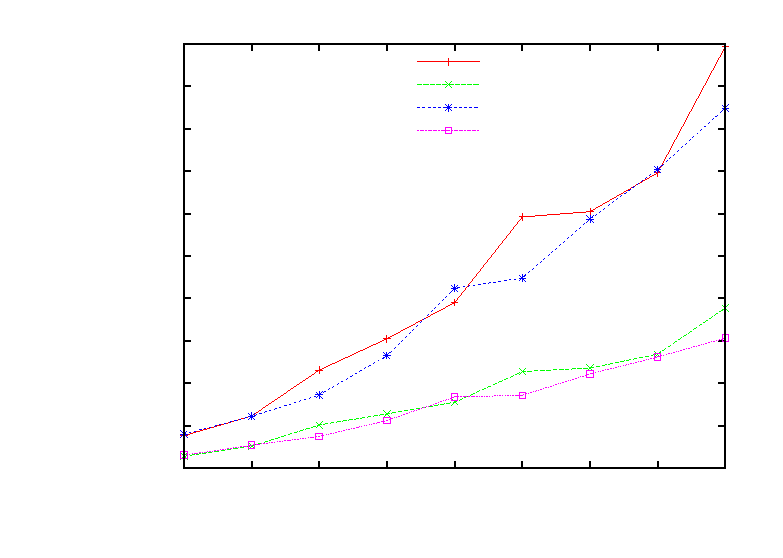
\includegraphics{L2L3NaiveVsPreallocatedSkewRankQueryCacheMisses}}%
    \gplfronttext
  \end{picture}%
\endgroup

\end{subfigure}
\end{figure}

\begin{figure}
\caption{Select Cache Misses on Wavelet Tree with increasing skew}
\label{fig:NaivePreallocatedSelectSkewCacheMisses}
\centering
\begin{subfigure}{\textwidth}
	\caption{Naive L1 vs. Preallocated L1}
	\label{fig:L1NaivePreallocatedSelectSkewCacheMisses}
	% GNUPLOT: LaTeX picture with Postscript
\begingroup
  \makeatletter
  \providecommand\color[2][]{%
    \GenericError{(gnuplot) \space\space\space\@spaces}{%
      Package color not loaded in conjunction with
      terminal option `colourtext'%
    }{See the gnuplot documentation for explanation.%
    }{Either use 'blacktext' in gnuplot or load the package
      color.sty in LaTeX.}%
    \renewcommand\color[2][]{}%
  }%
  \providecommand\includegraphics[2][]{%
    \GenericError{(gnuplot) \space\space\space\@spaces}{%
      Package graphicx or graphics not loaded%
    }{See the gnuplot documentation for explanation.%
    }{The gnuplot epslatex terminal needs graphicx.sty or graphics.sty.}%
    \renewcommand\includegraphics[2][]{}%
  }%
  \providecommand\rotatebox[2]{#2}%
  \@ifundefined{ifGPcolor}{%
    \newif\ifGPcolor
    \GPcolortrue
  }{}%
  \@ifundefined{ifGPblacktext}{%
    \newif\ifGPblacktext
    \GPblacktexttrue
  }{}%
  % define a \g@addto@macro without @ in the name:
  \let\gplgaddtomacro\g@addto@macro
  % define empty templates for all commands taking text:
  \gdef\gplbacktext{}%
  \gdef\gplfronttext{}%
  \makeatother
  \ifGPblacktext
    % no textcolor at all
    \def\colorrgb#1{}%
    \def\colorgray#1{}%
  \else
    % gray or color?
    \ifGPcolor
      \def\colorrgb#1{\color[rgb]{#1}}%
      \def\colorgray#1{\color[gray]{#1}}%
      \expandafter\def\csname LTw\endcsname{\color{white}}%
      \expandafter\def\csname LTb\endcsname{\color{black}}%
      \expandafter\def\csname LTa\endcsname{\color{black}}%
      \expandafter\def\csname LT0\endcsname{\color[rgb]{1,0,0}}%
      \expandafter\def\csname LT1\endcsname{\color[rgb]{0,1,0}}%
      \expandafter\def\csname LT2\endcsname{\color[rgb]{0,0,1}}%
      \expandafter\def\csname LT3\endcsname{\color[rgb]{1,0,1}}%
      \expandafter\def\csname LT4\endcsname{\color[rgb]{0,1,1}}%
      \expandafter\def\csname LT5\endcsname{\color[rgb]{1,1,0}}%
      \expandafter\def\csname LT6\endcsname{\color[rgb]{0,0,0}}%
      \expandafter\def\csname LT7\endcsname{\color[rgb]{1,0.3,0}}%
      \expandafter\def\csname LT8\endcsname{\color[rgb]{0.5,0.5,0.5}}%
    \else
      % gray
      \def\colorrgb#1{\color{black}}%
      \def\colorgray#1{\color[gray]{#1}}%
      \expandafter\def\csname LTw\endcsname{\color{white}}%
      \expandafter\def\csname LTb\endcsname{\color{black}}%
      \expandafter\def\csname LTa\endcsname{\color{black}}%
      \expandafter\def\csname LT0\endcsname{\color{black}}%
      \expandafter\def\csname LT1\endcsname{\color{black}}%
      \expandafter\def\csname LT2\endcsname{\color{black}}%
      \expandafter\def\csname LT3\endcsname{\color{black}}%
      \expandafter\def\csname LT4\endcsname{\color{black}}%
      \expandafter\def\csname LT5\endcsname{\color{black}}%
      \expandafter\def\csname LT6\endcsname{\color{black}}%
      \expandafter\def\csname LT7\endcsname{\color{black}}%
      \expandafter\def\csname LT8\endcsname{\color{black}}%
    \fi
  \fi
  \setlength{\unitlength}{0.0500bp}%
  \begin{picture}(7200.00,5040.00)%
    \gplgaddtomacro\gplbacktext{%
      \csname LTb\endcsname%
      \put(1474,704){\makebox(0,0)[r]{\strut{} 2e+07}}%
      \put(1474,1383){\makebox(0,0)[r]{\strut{} 4e+07}}%
      \put(1474,2061){\makebox(0,0)[r]{\strut{} 6e+07}}%
      \put(1474,2740){\makebox(0,0)[r]{\strut{} 8e+07}}%
      \put(1474,3418){\makebox(0,0)[r]{\strut{} 1e+08}}%
      \put(1474,4097){\makebox(0,0)[r]{\strut{} 1.2e+08}}%
      \put(1474,4775){\makebox(0,0)[r]{\strut{} 1.4e+08}}%
      \put(1606,484){\makebox(0,0){\strut{} 2}}%
      \put(2348,484){\makebox(0,0){\strut{} 4}}%
      \put(3091,484){\makebox(0,0){\strut{} 6}}%
      \put(3833,484){\makebox(0,0){\strut{} 8}}%
      \put(4576,484){\makebox(0,0){\strut{} 10}}%
      \put(5318,484){\makebox(0,0){\strut{} 12}}%
      \put(6061,484){\makebox(0,0){\strut{} 14}}%
      \put(6803,484){\makebox(0,0){\strut{} 16}}%
      \put(176,2739){\rotatebox{-270}{\makebox(0,0){\strut{}Cache Misses}}}%
      \put(4204,154){\makebox(0,0){\strut{}Skew}}%
    }%
    \gplgaddtomacro\gplfronttext{%
      \csname LTb\endcsname%
      \put(3718,4602){\makebox(0,0)[r]{\strut{}Naive L1}}%
      \csname LTb\endcsname%
      \put(3718,4382){\makebox(0,0)[r]{\strut{}Preallocated L1}}%
    }%
    \gplbacktext
    \put(0,0){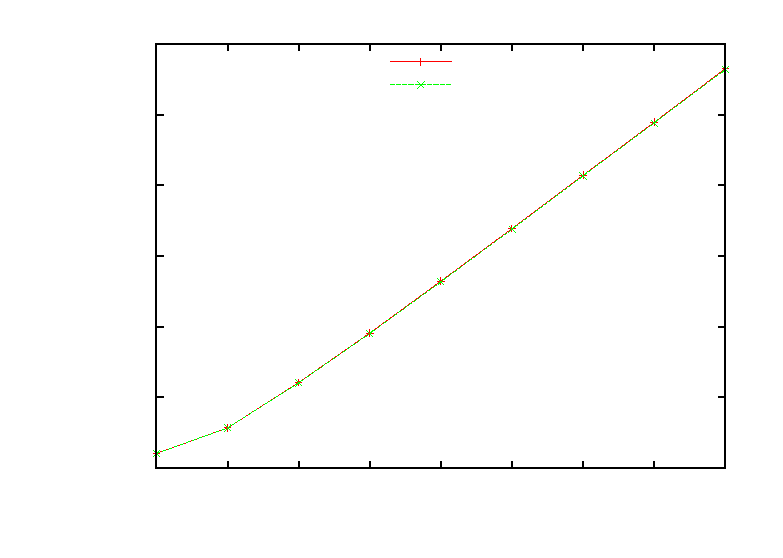
\includegraphics{L1NaiveVsPreallocatedSkewSelectQueryCacheMisses}}%
    \gplfronttext
  \end{picture}%
\endgroup

	\vspace*{5 mm}
\end{subfigure}
\begin{subfigure}{\textwidth}
	\caption{Naive L2, L3 vs. Preallocated L2, L3}
	\label{fig:L2L3NaivePreallocatedSelectSkewCacheMisses}
 	% GNUPLOT: LaTeX picture with Postscript
\begingroup
  \makeatletter
  \providecommand\color[2][]{%
    \GenericError{(gnuplot) \space\space\space\@spaces}{%
      Package color not loaded in conjunction with
      terminal option `colourtext'%
    }{See the gnuplot documentation for explanation.%
    }{Either use 'blacktext' in gnuplot or load the package
      color.sty in LaTeX.}%
    \renewcommand\color[2][]{}%
  }%
  \providecommand\includegraphics[2][]{%
    \GenericError{(gnuplot) \space\space\space\@spaces}{%
      Package graphicx or graphics not loaded%
    }{See the gnuplot documentation for explanation.%
    }{The gnuplot epslatex terminal needs graphicx.sty or graphics.sty.}%
    \renewcommand\includegraphics[2][]{}%
  }%
  \providecommand\rotatebox[2]{#2}%
  \@ifundefined{ifGPcolor}{%
    \newif\ifGPcolor
    \GPcolortrue
  }{}%
  \@ifundefined{ifGPblacktext}{%
    \newif\ifGPblacktext
    \GPblacktexttrue
  }{}%
  % define a \g@addto@macro without @ in the name:
  \let\gplgaddtomacro\g@addto@macro
  % define empty templates for all commands taking text:
  \gdef\gplbacktext{}%
  \gdef\gplfronttext{}%
  \makeatother
  \ifGPblacktext
    % no textcolor at all
    \def\colorrgb#1{}%
    \def\colorgray#1{}%
  \else
    % gray or color?
    \ifGPcolor
      \def\colorrgb#1{\color[rgb]{#1}}%
      \def\colorgray#1{\color[gray]{#1}}%
      \expandafter\def\csname LTw\endcsname{\color{white}}%
      \expandafter\def\csname LTb\endcsname{\color{black}}%
      \expandafter\def\csname LTa\endcsname{\color{black}}%
      \expandafter\def\csname LT0\endcsname{\color[rgb]{1,0,0}}%
      \expandafter\def\csname LT1\endcsname{\color[rgb]{0,1,0}}%
      \expandafter\def\csname LT2\endcsname{\color[rgb]{0,0,1}}%
      \expandafter\def\csname LT3\endcsname{\color[rgb]{1,0,1}}%
      \expandafter\def\csname LT4\endcsname{\color[rgb]{0,1,1}}%
      \expandafter\def\csname LT5\endcsname{\color[rgb]{1,1,0}}%
      \expandafter\def\csname LT6\endcsname{\color[rgb]{0,0,0}}%
      \expandafter\def\csname LT7\endcsname{\color[rgb]{1,0.3,0}}%
      \expandafter\def\csname LT8\endcsname{\color[rgb]{0.5,0.5,0.5}}%
    \else
      % gray
      \def\colorrgb#1{\color{black}}%
      \def\colorgray#1{\color[gray]{#1}}%
      \expandafter\def\csname LTw\endcsname{\color{white}}%
      \expandafter\def\csname LTb\endcsname{\color{black}}%
      \expandafter\def\csname LTa\endcsname{\color{black}}%
      \expandafter\def\csname LT0\endcsname{\color{black}}%
      \expandafter\def\csname LT1\endcsname{\color{black}}%
      \expandafter\def\csname LT2\endcsname{\color{black}}%
      \expandafter\def\csname LT3\endcsname{\color{black}}%
      \expandafter\def\csname LT4\endcsname{\color{black}}%
      \expandafter\def\csname LT5\endcsname{\color{black}}%
      \expandafter\def\csname LT6\endcsname{\color{black}}%
      \expandafter\def\csname LT7\endcsname{\color{black}}%
      \expandafter\def\csname LT8\endcsname{\color{black}}%
    \fi
  \fi
  \setlength{\unitlength}{0.0500bp}%
  \begin{picture}(7200.00,5040.00)%
    \gplgaddtomacro\gplbacktext{%
      \csname LTb\endcsname%
      \put(1474,704){\makebox(0,0)[r]{\strut{} 0}}%
      \put(1474,1286){\makebox(0,0)[r]{\strut{} 2e+06}}%
      \put(1474,1867){\makebox(0,0)[r]{\strut{} 4e+06}}%
      \put(1474,2449){\makebox(0,0)[r]{\strut{} 6e+06}}%
      \put(1474,3030){\makebox(0,0)[r]{\strut{} 8e+06}}%
      \put(1474,3612){\makebox(0,0)[r]{\strut{} 1e+07}}%
      \put(1474,4193){\makebox(0,0)[r]{\strut{} 1.2e+07}}%
      \put(1474,4775){\makebox(0,0)[r]{\strut{} 1.4e+07}}%
      \put(1606,484){\makebox(0,0){\strut{} 2}}%
      \put(2348,484){\makebox(0,0){\strut{} 4}}%
      \put(3091,484){\makebox(0,0){\strut{} 6}}%
      \put(3833,484){\makebox(0,0){\strut{} 8}}%
      \put(4576,484){\makebox(0,0){\strut{} 10}}%
      \put(5318,484){\makebox(0,0){\strut{} 12}}%
      \put(6061,484){\makebox(0,0){\strut{} 14}}%
      \put(6803,484){\makebox(0,0){\strut{} 16}}%
      \put(176,2739){\rotatebox{-270}{\makebox(0,0){\strut{}Cache Misses}}}%
      \put(4204,154){\makebox(0,0){\strut{}Skew}}%
    }%
    \gplgaddtomacro\gplfronttext{%
      \csname LTb\endcsname%
      \put(3718,4602){\makebox(0,0)[r]{\strut{}Naive L2}}%
      \csname LTb\endcsname%
      \put(3718,4382){\makebox(0,0)[r]{\strut{}Naive L3}}%
      \csname LTb\endcsname%
      \put(3718,4162){\makebox(0,0)[r]{\strut{}Preallocated L2}}%
      \csname LTb\endcsname%
      \put(3718,3942){\makebox(0,0)[r]{\strut{}Preallocated L3}}%
    }%
    \gplbacktext
    \put(0,0){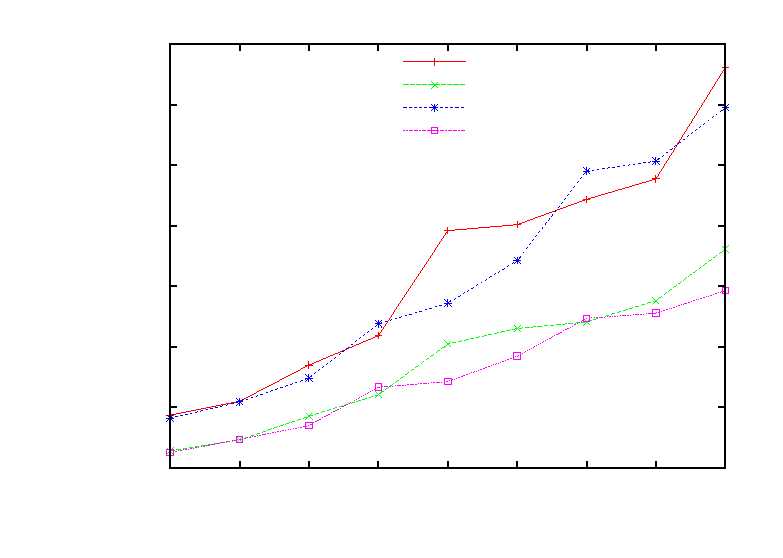
\includegraphics{L2L3NaiveVsPreallocatedSkewSelectQueryCacheMisses}}%
    \gplfronttext
  \end{picture}%
\endgroup

\end{subfigure}
\end{figure}


\paragraph{TLB}

\begin{figure}
\caption{Rank TLB}
\label{fig:NaiveVsPreallocatedSkewRankQueryTLB}
% GNUPLOT: LaTeX picture with Postscript
\begingroup
  \makeatletter
  \providecommand\color[2][]{%
    \GenericError{(gnuplot) \space\space\space\@spaces}{%
      Package color not loaded in conjunction with
      terminal option `colourtext'%
    }{See the gnuplot documentation for explanation.%
    }{Either use 'blacktext' in gnuplot or load the package
      color.sty in LaTeX.}%
    \renewcommand\color[2][]{}%
  }%
  \providecommand\includegraphics[2][]{%
    \GenericError{(gnuplot) \space\space\space\@spaces}{%
      Package graphicx or graphics not loaded%
    }{See the gnuplot documentation for explanation.%
    }{The gnuplot epslatex terminal needs graphicx.sty or graphics.sty.}%
    \renewcommand\includegraphics[2][]{}%
  }%
  \providecommand\rotatebox[2]{#2}%
  \@ifundefined{ifGPcolor}{%
    \newif\ifGPcolor
    \GPcolortrue
  }{}%
  \@ifundefined{ifGPblacktext}{%
    \newif\ifGPblacktext
    \GPblacktexttrue
  }{}%
  % define a \g@addto@macro without @ in the name:
  \let\gplgaddtomacro\g@addto@macro
  % define empty templates for all commands taking text:
  \gdef\gplbacktext{}%
  \gdef\gplfronttext{}%
  \makeatother
  \ifGPblacktext
    % no textcolor at all
    \def\colorrgb#1{}%
    \def\colorgray#1{}%
  \else
    % gray or color?
    \ifGPcolor
      \def\colorrgb#1{\color[rgb]{#1}}%
      \def\colorgray#1{\color[gray]{#1}}%
      \expandafter\def\csname LTw\endcsname{\color{white}}%
      \expandafter\def\csname LTb\endcsname{\color{black}}%
      \expandafter\def\csname LTa\endcsname{\color{black}}%
      \expandafter\def\csname LT0\endcsname{\color[rgb]{1,0,0}}%
      \expandafter\def\csname LT1\endcsname{\color[rgb]{0,1,0}}%
      \expandafter\def\csname LT2\endcsname{\color[rgb]{0,0,1}}%
      \expandafter\def\csname LT3\endcsname{\color[rgb]{1,0,1}}%
      \expandafter\def\csname LT4\endcsname{\color[rgb]{0,1,1}}%
      \expandafter\def\csname LT5\endcsname{\color[rgb]{1,1,0}}%
      \expandafter\def\csname LT6\endcsname{\color[rgb]{0,0,0}}%
      \expandafter\def\csname LT7\endcsname{\color[rgb]{1,0.3,0}}%
      \expandafter\def\csname LT8\endcsname{\color[rgb]{0.5,0.5,0.5}}%
    \else
      % gray
      \def\colorrgb#1{\color{black}}%
      \def\colorgray#1{\color[gray]{#1}}%
      \expandafter\def\csname LTw\endcsname{\color{white}}%
      \expandafter\def\csname LTb\endcsname{\color{black}}%
      \expandafter\def\csname LTa\endcsname{\color{black}}%
      \expandafter\def\csname LT0\endcsname{\color{black}}%
      \expandafter\def\csname LT1\endcsname{\color{black}}%
      \expandafter\def\csname LT2\endcsname{\color{black}}%
      \expandafter\def\csname LT3\endcsname{\color{black}}%
      \expandafter\def\csname LT4\endcsname{\color{black}}%
      \expandafter\def\csname LT5\endcsname{\color{black}}%
      \expandafter\def\csname LT6\endcsname{\color{black}}%
      \expandafter\def\csname LT7\endcsname{\color{black}}%
      \expandafter\def\csname LT8\endcsname{\color{black}}%
    \fi
  \fi
  \setlength{\unitlength}{0.0500bp}%
  \begin{picture}(7200.00,5040.00)%
    \gplgaddtomacro\gplbacktext{%
      \csname LTb\endcsname%
      \put(1210,704){\makebox(0,0)[r]{\strut{} 0}}%
      \put(1210,1286){\makebox(0,0)[r]{\strut{} 10000}}%
      \put(1210,1867){\makebox(0,0)[r]{\strut{} 20000}}%
      \put(1210,2449){\makebox(0,0)[r]{\strut{} 30000}}%
      \put(1210,3030){\makebox(0,0)[r]{\strut{} 40000}}%
      \put(1210,3612){\makebox(0,0)[r]{\strut{} 50000}}%
      \put(1210,4193){\makebox(0,0)[r]{\strut{} 60000}}%
      \put(1210,4775){\makebox(0,0)[r]{\strut{} 70000}}%
      \put(1342,484){\makebox(0,0){\strut{} 2}}%
      \put(2025,484){\makebox(0,0){\strut{} 2.5}}%
      \put(2707,484){\makebox(0,0){\strut{} 3}}%
      \put(3390,484){\makebox(0,0){\strut{} 3.5}}%
      \put(4073,484){\makebox(0,0){\strut{} 4}}%
      \put(4755,484){\makebox(0,0){\strut{} 4.5}}%
      \put(5438,484){\makebox(0,0){\strut{} 5}}%
      \put(6120,484){\makebox(0,0){\strut{} 5.5}}%
      \put(6803,484){\makebox(0,0){\strut{} 6}}%
      \put(176,2739){\rotatebox{-270}{\makebox(0,0){\strut{}TLB}}}%
      \put(4072,154){\makebox(0,0){\strut{}Skew}}%
    }%
    \gplgaddtomacro\gplfronttext{%
      \csname LTb\endcsname%
      \put(3058,4602){\makebox(0,0)[r]{\strut{}Naive}}%
    }%
    \gplbacktext
    \put(0,0){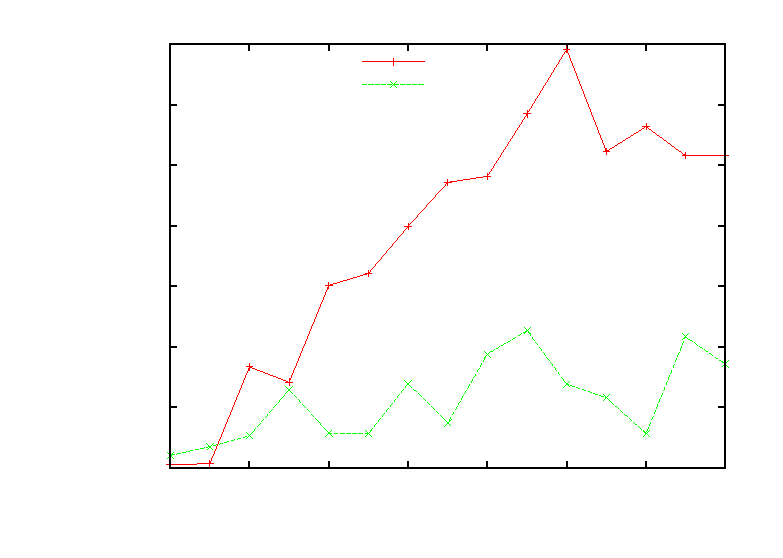
\includegraphics{NaiveVsPreallocatedSkewRankQueryTLB}}%
    \gplfronttext
  \end{picture}%
\endgroup

\end{figure}

\begin{figure}
\caption{Select TLB}
\label{fig:NaiveVsPreallocatedSkewSelectQueryTLB}
% GNUPLOT: LaTeX picture with Postscript
\begingroup
  \makeatletter
  \providecommand\color[2][]{%
    \GenericError{(gnuplot) \space\space\space\@spaces}{%
      Package color not loaded in conjunction with
      terminal option `colourtext'%
    }{See the gnuplot documentation for explanation.%
    }{Either use 'blacktext' in gnuplot or load the package
      color.sty in LaTeX.}%
    \renewcommand\color[2][]{}%
  }%
  \providecommand\includegraphics[2][]{%
    \GenericError{(gnuplot) \space\space\space\@spaces}{%
      Package graphicx or graphics not loaded%
    }{See the gnuplot documentation for explanation.%
    }{The gnuplot epslatex terminal needs graphicx.sty or graphics.sty.}%
    \renewcommand\includegraphics[2][]{}%
  }%
  \providecommand\rotatebox[2]{#2}%
  \@ifundefined{ifGPcolor}{%
    \newif\ifGPcolor
    \GPcolortrue
  }{}%
  \@ifundefined{ifGPblacktext}{%
    \newif\ifGPblacktext
    \GPblacktexttrue
  }{}%
  % define a \g@addto@macro without @ in the name:
  \let\gplgaddtomacro\g@addto@macro
  % define empty templates for all commands taking text:
  \gdef\gplbacktext{}%
  \gdef\gplfronttext{}%
  \makeatother
  \ifGPblacktext
    % no textcolor at all
    \def\colorrgb#1{}%
    \def\colorgray#1{}%
  \else
    % gray or color?
    \ifGPcolor
      \def\colorrgb#1{\color[rgb]{#1}}%
      \def\colorgray#1{\color[gray]{#1}}%
      \expandafter\def\csname LTw\endcsname{\color{white}}%
      \expandafter\def\csname LTb\endcsname{\color{black}}%
      \expandafter\def\csname LTa\endcsname{\color{black}}%
      \expandafter\def\csname LT0\endcsname{\color[rgb]{1,0,0}}%
      \expandafter\def\csname LT1\endcsname{\color[rgb]{0,1,0}}%
      \expandafter\def\csname LT2\endcsname{\color[rgb]{0,0,1}}%
      \expandafter\def\csname LT3\endcsname{\color[rgb]{1,0,1}}%
      \expandafter\def\csname LT4\endcsname{\color[rgb]{0,1,1}}%
      \expandafter\def\csname LT5\endcsname{\color[rgb]{1,1,0}}%
      \expandafter\def\csname LT6\endcsname{\color[rgb]{0,0,0}}%
      \expandafter\def\csname LT7\endcsname{\color[rgb]{1,0.3,0}}%
      \expandafter\def\csname LT8\endcsname{\color[rgb]{0.5,0.5,0.5}}%
    \else
      % gray
      \def\colorrgb#1{\color{black}}%
      \def\colorgray#1{\color[gray]{#1}}%
      \expandafter\def\csname LTw\endcsname{\color{white}}%
      \expandafter\def\csname LTb\endcsname{\color{black}}%
      \expandafter\def\csname LTa\endcsname{\color{black}}%
      \expandafter\def\csname LT0\endcsname{\color{black}}%
      \expandafter\def\csname LT1\endcsname{\color{black}}%
      \expandafter\def\csname LT2\endcsname{\color{black}}%
      \expandafter\def\csname LT3\endcsname{\color{black}}%
      \expandafter\def\csname LT4\endcsname{\color{black}}%
      \expandafter\def\csname LT5\endcsname{\color{black}}%
      \expandafter\def\csname LT6\endcsname{\color{black}}%
      \expandafter\def\csname LT7\endcsname{\color{black}}%
      \expandafter\def\csname LT8\endcsname{\color{black}}%
    \fi
  \fi
  \setlength{\unitlength}{0.0500bp}%
  \begin{picture}(7200.00,5040.00)%
    \gplgaddtomacro\gplbacktext{%
      \csname LTb\endcsname%
      \put(1474,704){\makebox(0,0)[r]{\strut{} 0}}%
      \put(1474,1383){\makebox(0,0)[r]{\strut{} 200000}}%
      \put(1474,2061){\makebox(0,0)[r]{\strut{} 400000}}%
      \put(1474,2740){\makebox(0,0)[r]{\strut{} 600000}}%
      \put(1474,3418){\makebox(0,0)[r]{\strut{} 800000}}%
      \put(1474,4097){\makebox(0,0)[r]{\strut{} 1e+06}}%
      \put(1474,4775){\makebox(0,0)[r]{\strut{} 1.2e+06}}%
      \put(1606,484){\makebox(0,0){\strut{} 2}}%
      \put(2348,484){\makebox(0,0){\strut{} 4}}%
      \put(3091,484){\makebox(0,0){\strut{} 6}}%
      \put(3833,484){\makebox(0,0){\strut{} 8}}%
      \put(4576,484){\makebox(0,0){\strut{} 10}}%
      \put(5318,484){\makebox(0,0){\strut{} 12}}%
      \put(6061,484){\makebox(0,0){\strut{} 14}}%
      \put(6803,484){\makebox(0,0){\strut{} 16}}%
      \put(176,2739){\rotatebox{-270}{\makebox(0,0){\strut{}TLB}}}%
      \put(4204,154){\makebox(0,0){\strut{}Skew}}%
    }%
    \gplgaddtomacro\gplfronttext{%
      \csname LTb\endcsname%
      \put(3322,4602){\makebox(0,0)[r]{\strut{}Naive}}%
      \csname LTb\endcsname%
      \put(3322,4382){\makebox(0,0)[r]{\strut{}Preallocated}}%
    }%
    \gplbacktext
    \put(0,0){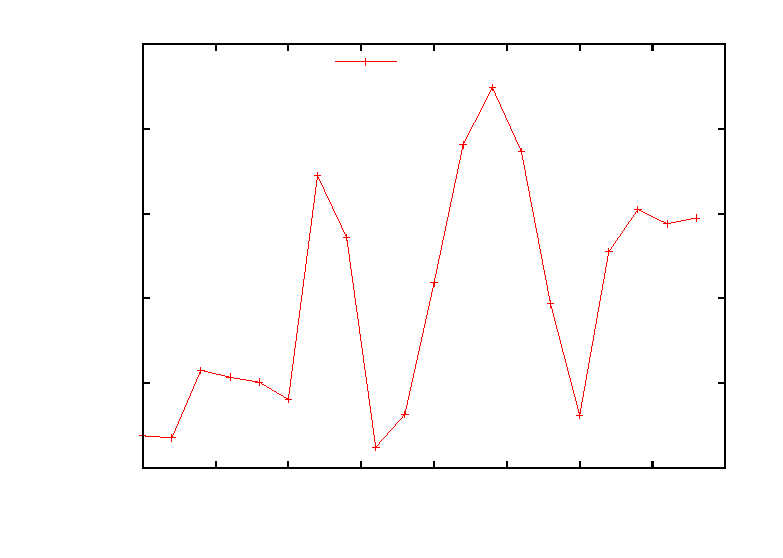
\includegraphics{NaiveVsPreallocatedSkewSelectQueryTLB}}%
    \gplfronttext
  \end{picture}%
\endgroup

\end{figure}



\subsubsection{Why controlled memory is not better than uncontrolled memory}
When we look at the graphs for cache misses and branch mis-predictions we can see that the difference between controlled and uncontrolled memory management is very small which fits very well with the fact that the query times are very close.
The cache misses for \textit{Level 1} (when comparing the two construction methods) are almost exactly equal while \textit{Level 2} and \textit{Level 3} cache misses varies a bit as shown in figure ~\ref{fig:NaivePreallocatedRankSkewCacheMisses} and \ref{fig:NaivePreallocatedSelectSkewCacheMisses}
This is because the size of the caches are larger in higher levels than in lower levels and \textit{Level 1} gets filled up much faster than \textit{Level 2} and \textit{Level 3} resulting in more \textit{Level 1} cache misses.

It can also explain why the difference in \textit{Level 1} cache misses is so small. 
The \textit{Level 1} cache simply gets filled up quickly and is then often missed. \textit{Level 2} and \textit{Level 3}are larger, which means that they do not reach their limit as quickly, resulting in fewer and more varied cache miss values.



Controlling the memory is in essence not better than letting the OS control it, which indicates that the effect of how we control memory is equal to the effect of how OS does it.







